\section{Conditioning on survival}
\label{sec:qsd}

Absorption is often inevitable, as it is here for $p<\tfrac12$, and yet long before it
occurs a process may settle into a distribution that no longer changes with time --- a
distribution of the population \emph{given} that absorption has not yet happened. This
is \emph{quasi-stationarity}, and the limit it describes is the quasi-stationary, or
Yaglom, distribution \cite{Yaglom1947,Athreya1972}. This section establishes it for the
binary Galton--Watson process by computing the limiting conditional mean and variance,
and in doing so it produces the constant that the rest of the chapter is about.

\subsection{The survival probability at late times}
\label{sec:lateS}

Everything follows from the decay of $S_n$. Take $p<\tfrac12$, so that death of an
individual is more probable than its division. Then $S_n\to0$, and as it does so the
quadratic term in
\begin{equation*}
S_{n+1} = 2pS_n - pS_n^2
\end{equation*}
becomes negligible beside the linear one. The recursion is therefore increasingly well
approximated by the linear map
\begin{equation}
\label{eq:attenuated}
S_{n+1} \approx 2p\,S_n,
\end{equation}
whose solution is a pure geometric. The late-time behaviour of the survival probability
is accordingly
\begin{equation}
\label{eq:lateS}
S_n \sim A(p)\,(2p)^n \qquad(n\to\infty),
\qquad
A(p) = \lim_{n\to\infty}\frac{S_n}{(2p)^n},
\end{equation}
and the whole of the nonlinearity has been pushed into the single constant $A(p)$. That
constant records the cumulative effect of the quadratic term over the early generations,
before the linear regime of \cref{eq:attenuated} takes hold; it is what the process
remembers of its own beginning. The limit exists and is finite and strictly positive for
$p\in[0,\tfrac12)$, a fact proved by an infinite product in \cref{sec:product} and
sharpened to $A(p)\in(0,\tfrac12]$ in \cref{sec:Abounds}.

\begin{remark}
\label{rem:asymptotic}
\Cref{eq:lateS} is an asymptotic equivalence, not an identity. For $p<\tfrac12$ the
limit of $S_n$ is $0$, and one must not write $\lim_n S_n = A(p)(2p)^n$, whose
right-hand side still depends on $n$. What converges is the ratio $S_n/(2p)^n$.
\end{remark}

\subsection{The conditional mean}
\label{sec:condmean}

Split the expected population size into contributions from surviving and extinct
realisations:
\begin{equation*}
\mean{\zz_n}
= \pr{\zz_n=0}\,\cancelto{0}{\mean{\zz_n\mid\zz_n=0}}
+ \pr{\zz_n>0}\,\mean{\zz_n\mid\zz_n>0}.
\end{equation*}
The first term vanishes identically, so with $\pr{\zz_n>0}=S_n$ and
$\mean{\zz_n}=(2p)^n$ from \cref{eq:meanZn},
\begin{equation}
\label{eq:condmeandef}
\mean{\zz_n\mid\zz_n>0} = \frac{\mean{\zz_n}}{S_n} = \frac{(2p)^n}{S_n}.
\end{equation}
The numerator is known exactly and the content sits entirely in the denominator, which
\cref{eq:lateS} supplies:
\begin{equation}
\label{eq:qsmean}
\mean{\zz_n\mid\zz_n>0}
\;\xrightarrow[n\to\infty]{}\;
\frac{(2p)^n}{A(p)(2p)^n} = \frac{1}{A(p)}.
\end{equation}
The geometric factors cancel exactly. At late times the surviving population therefore
has a constant expected size, and that size is the reciprocal of $A(p)$; for this reason
$1/A(p)$ is called the \emph{quasi-stationary mean} below. Two exponentially small
quantities have been divided into one another to leave something of order unity, which
is what conditioning on a vanishing event generally does and why the unconditional mean
was so uninformative.

\Cref{fig:condmean} shows the convergence, and also shows the obstacle that
\cref{sec:Ap} will have to deal with: the closer $p$ lies to $\tfrac12$, the higher the
plateau and the more generations are needed to reach it.

\begin{figure}[ht]
\centering
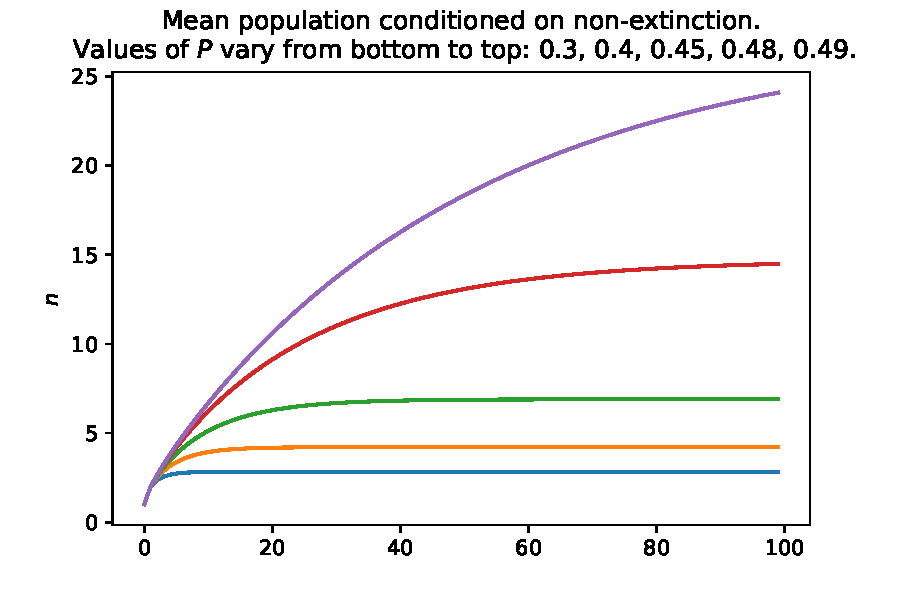
\includegraphics[width=0.78\textwidth]{figures/IMG_ch3/conditionalMean.pdf}
\caption{The conditional mean $(2p)^n/S_n$ against generation number $n$, with $S_n$
obtained by iterating \cref{eq:SnIter}. From bottom to top,
$p=0.3,\,0.4,\,0.45,\,0.48,\,0.49$. Each curve approaches the constant $1/A(p)$, whose
values are $2.825$, $4.208$, $6.893$, $14.703$ and $27.476$, computed as in
\cref{sec:practical}. The lowest three have essentially converged by $n=100$; the
$p=0.49$ curve has reached only $24.1$ of its limiting $27.5$, which is an early sign of
the near-critical slowdown quantified in \cref{tab:Avals}. (The vertical axis is
mislabelled $n$ in the original plotting script; the quantity plotted is the conditional
mean.)}
\label{fig:condmean}
\end{figure}

\subsection{The conditional variance}
\label{sec:variance}

A stable mean is not yet quasi-stationarity. To show that the conditional
\emph{distribution} settles we need at least the second moment, and obtaining it is a
useful exercise in the composition structure of \cref{eq:phicomp}.

\subsubsection{The second moment}

Work with the moment generating function $M_n(t) = \mean{\ee^{t\zz_n}}$, which is the
\pgf{} evaluated on the exponential,
\begin{equation}
\label{eq:mgfdef}
M_n(t) = \phi_n\lrb{\ee^{t}},
\qquad
\mean{\zz_n^{\,k}} = M_n^{(k)}(0),
\end{equation}
and note the two facts that make the calculation short. First, $M_n(0)=1$ for every $n$.
Second, the offspring \pgf{} \cref{eq:pgfbinary} has the linear derivative
$\phi'(z) = 2pz$. Since $\phi_n = \phi\circ\phi_{n-1}$, the chain rule gives
\begin{equation}
\label{eq:mgfrec}
M_n'(t) = \phi'\lrb{\phi_{n-1}(\ee^t)}\,M_{n-1}'(t) = 2p\,M_{n-1}(t)\,M_{n-1}'(t),
\end{equation}
a recursion in which the derivative of the composition never has to be expanded.
Evaluating \cref{eq:mgfrec} at $t=0$ recovers the mean, $M_n'(0) = 2p\,M_{n-1}'(0)$ and
hence $M_n'(0) = (2p)^n$, as it must by \cref{eq:meanZn}. Differentiating
\cref{eq:mgfrec} once more,
\begin{equation*}
M_n''(t) = 2p\lrb{\bigl(M_{n-1}'(t)\bigr)^2 + M_{n-1}(t)M_{n-1}''(t)},
\end{equation*}
and setting $t=0$ turns this into a linear recursion for the second moments. Writing
$m_n = \mean{\zz_n^2} = M_n''(0)$ and $\mu=2p$,
\begin{equation}
\label{eq:secondrec}
m_n = \mu\,\mu^{2(n-1)} + \mu\,m_{n-1} = \mu^{2n-1} + \mu\,m_{n-1},
\qquad m_0 = 1 .
\end{equation}
Unrolling \cref{eq:secondrec} gives $m_n = \mu^n + \sum_{j=1}^{n}\mu^{n-j}\mu^{2j-1}
= \mu^n\bigl(1+\sum_{i=0}^{n-1}\mu^i\bigr)$, and summing the finite geometric series,
\begin{equation}
\label{eq:secondMoment}
\mean{\zz_n^2}
= (2p)^n\lrbs{1 + \frac{1-(2p)^n}{1-2p}}
= (2p)^n\lrb{1+\frac{1}{1-2p}} - (2p)^{2n}\lrb{\frac{1}{1-2p}} .
\end{equation}
At $n=1$ the right-hand side returns $2p + (2p-4p^2)/(1-2p) = 4p$, which is
$\mean{\zz_1^2}$ for the binary offspring law, so the signs are as they should be.

\subsubsection{Late-time behaviour}

Subtracting $\mean{\zz_n}^2 = (2p)^{2n}$ from \cref{eq:secondMoment} gives a variance
that factorises neatly,
\begin{equation}
\label{eq:uncondvar}
\text{Var}(\zz_n) = \lrb{1+\frac{1}{1-2p}}\lrb{(2p)^n - (2p)^{2n}},
\end{equation}
so for $2p<1$ the variance decays geometrically like $(2p)^n$, at the same rate as the
mean. It is tempting to read stationarity of the conditional variance directly off
\cref{eq:uncondvar}, but that would be too quick: the conditional variance is not the
unconditional one divided by anything simple. The safe route is through the conditional
moments themselves. Dividing by $S_n$ and using \cref{eq:lateS}, with the $(2p)^{2n}$
terms negligible beside $(2p)^n$,
\begin{align*}
\mean{\zz_n^2\mid\zz_n>0} &= \frac{\mean{\zz_n^2}}{S_n}
\;\xrightarrow{n\to\infty}\;
\frac{1}{A}\lrb{1+\frac{1}{1-2p}},\\[4pt]
\mean{\zz_n\mid\zz_n>0} &= \frac{\mean{\zz_n}}{S_n}
\;\xrightarrow{n\to\infty}\;
\frac{1}{A} .
\end{align*}
Both limits are finite, so the conditional variance tends to a constant,
\begin{equation}
\label{eq:condvar}
\text{Var}(\zz_n\mid\zz_n>0)
\;\longrightarrow\;
\frac{1}{A}\lrb{1+\frac{1}{1-2p}} - \frac{1}{A^2} .
\end{equation}
The first two moments of the conditional population therefore both stabilise, and the
same argument carried to higher moments gives the full quasi-stationary distribution.
As a check on \cref{eq:condvar}, let $p\to0$: there $A\to\tfrac12$ and the bracket tends
to $2$, so the limiting conditional variance is $2\cdot2-4=0$. Deep in the subcritical
regime a surviving population consists of exactly two individuals and has no spread at
all, which is the parity effect made precise in \cref{prop:parity}.

What matters for the rest of the chapter is that \cref{eq:qsmean,eq:condvar} are both
expressed in terms of $p$ and the single unknown constant $A(p)$. Everything now turns
on that constant.

\subsection{A continuum view of the survival recursion}
\label{sec:riccati}

Before attacking $A(p)$ directly it is worth recording a continuum approximation to
\cref{eq:SnIter}, both because it recurs later and because its failure is instructive.
Write $\varepsilon = 1-2p$ for the distance from criticality, so that the exact
difference is
\begin{equation}
\label{eq:Sdiff}
S_{n+1}-S_n = -\varepsilon S_n - pS_n^2 .
\end{equation}
For large $n$ the unit increment is small on the scale over which $S$ varies, and
replacing the left-hand side by a derivative gives a Riccati equation,
\begin{equation}
\label{eq:riccati}
\dda{S}{n} = -\varepsilon S - pS^2 .
\end{equation}
The substitution $u=1/S$ linearises it to $u' = \varepsilon u + p$, with solution
$u(n) = K\ee^{\varepsilon n} - p/\varepsilon$ and hence
\begin{equation}
\label{eq:riccatisol}
S(n) = \frac{\varepsilon}{K\varepsilon\,\ee^{\varepsilon n} - p},
\end{equation}
where $K$ is a constant of integration fixed by the initial condition. Both known
regimes are contained in \cref{eq:riccatisol}. Setting $\varepsilon=0$ recovers the
critical scaling $S\sim2/n$ of \cref{eq:twoovrn}; keeping $\varepsilon>0$ recovers the
geometric decay $S\sim A(2p)^n$ of \cref{eq:lateS}, since
$(2p)^n = \ee^{\,n\ln(1-\varepsilon)}$ agrees with $\ee^{-\varepsilon n}$ to leading
order in $\varepsilon$.

What \cref{eq:riccatisol} does not contain is $K$. The continuum approximation is valid
only once $n$ is large, whereas $K$ is determined by the early generations in which it
fails, and $K$ is --- up to the identification just made --- precisely $A(p)$. No
argument of this kind will produce it. \Cref{sec:asymptotic} shows how much can
nevertheless be extracted from \cref{eq:riccati} in the near-critical limit, where the
early generations occupy a vanishing fraction of the process's life.

\FloatBarrier
